\chapter{Redundancy under Discussion}\label{chap:redundancy}

\textbf{Abstract.} This chapter presents novel data derived from a redundant structure ($p\vee p \vee q$) \textit{via} the \textit{or}-to-\textit{if} tautology and core properties of disjunction (commutativity, associativity). The sentences at stake exhibit differing degrees of pragmatic oddness, which represents a challenge for existing theories of redundancy. Building on a new QuD-informed model of pragmatic oddness, we propose a solution covering almost all the cases at stake, and discuss how the remaining problematic cases might be solved assuming an incremental view of redundancy.


\section{Introduction}
The disjunctive sentences in (\ref{ex2:double-disjunctions}), which are logically related to each other \textit{via} applications of $\vee$-commutativity and $\vee$-associativity, appear sharply infelicitous.\footnote{More variants could be derived, for instance $q\vee(p\vee p)$. Here, we focus on the less obvious variants where two instances of $p$ do not directly combine together.} Such sentences can be seen as pragmatically odd, because they are all contextually equivalent to their complex disjunct, $p\vee q$ or $q \vee p$
\citep{Katzir2014}.
\begin{exe}
	\ex \textit{Context: Ido is supposed to present at Sinn und Bedeutung, but maybe he will not come in person.}\label{ex2:double-disjunctions}
	\begin{xlist}
		\ex[\#] {Either Ido is at SuB, or else he is at SuB or in Cambridge.\\ \hfill $\p\vee (\p \vee \q)$}\label{ex2:pv(pvq)}
		\ex[\#] {Either Ido is at SuB, or else he is in Cambridge or at SuB.\hfill $\p\vee (\q \vee \p)$}\label{ex2:pv(qvp)}
		\ex[\#] {Either Ido is at SuB or in Cambridge, or else he is at SuB.\hfill $(\p \vee \q) \vee \p$}\label{ex2:(pvq)vp}
		\ex[\#] {Either Ido is in Cambridge or at SuB, or else he is at SuB.\hfill $(\q \vee \p) \vee \p$}\label{ex2:(qvp)vp}
	\end{xlist}
	
\end{exe} 
(\ref{ex2:pv(pvq)-variants}-\ref{ex2:(qvp)vp-variants}) show variants of the sentences in (\ref{ex2:double-disjunctions}) obtained \textit{via} the \textit{or}-to-\textit{if} tautology. In each pair of sentences, the a. instances are derived by modifying the outer disjunction, while the the b. instances are derived by modifying the inner disjunction.\footnote{One could also apply the \textit{or}-to-\textit{if} tautology to \textit{both} the inner and the outer disjunction in the sentences in (\ref{ex2:double-disjunctions}). Nested conditionals however, are hard to judge. That is why we omit them in this introduction.}. Surprisingly, those variants exhibit different degrees of oddness: only (\ref{ex2:pv(nptq)}) and (\ref{ex2:(nptq)vp}) escape infelicity. This is unexpected given that all the sentences in (\ref{ex2:pv(pvq)-variants}-\ref{ex2:(qvp)vp-variants}) have same logical structure as the infelicitous sentences in (\ref{ex2:pv(pvq)}-\ref{ex2:(qvp)vp}), assuming implications are material. Particularly puzzling is the existence of a contrast \textit{between} the different b. examples in (\ref{ex2:pv(pvq)-variants}-\ref{ex2:(qvp)vp-variants}), which are derived from (\ref{ex2:pv(pvq)}-\ref{ex2:(qvp)vp}) using the \textit{same} operation.
\begin{exe}
	\ex Derived from (\ref{ex2:pv(pvq)}):
	\begin{xlist}
		\ex[\#] {If Ido is not at SuB then he is at SuB or in Cambridge.\\ $\neg \p \rightarrow (\p \vee \q)$}\label{ex2:npt(pvq)}
		\ex[] {Either Ido is at SuB or if he is not at SuB then he is in Cambridge.\\ \hfill $\p \vee (\neg \p \rightarrow \q)$}\label{ex2:pv(nptq)}
	\end{xlist}\label{ex2:pv(pvq)-variants}
	\ex Derived from (\ref{ex2:pv(qvp)}):
	\begin{xlist}
		\ex[\#] {If Ido is not at SuB then he is in Cambridge or at SuB.\\ \hfill $\neg \p \rightarrow (\q \vee \p)$}\label{ex2:npt(qvp)}
		\ex[\#] {Either Ido is at SuB or if he is not in Cambridge then he is at SuB.\\ \hfill $\p \vee (\neg \q \rightarrow \p)$}\label{ex2:pv(nqtp)}
	\end{xlist}\label{ex2:pv(qvp)-variants}
	\ex Derived from (\ref{ex2:(pvq)vp}):
	\begin{xlist}
		\ex[\#] {If it's not true that Ido is at SuB or in Cambridge, then he is at SuB.\\ \hfill $\neg (\p \vee \q) \rightarrow \p$}\label{ex2:n(pvq)tp}
		\ex[?] {Either Ido is in Cambridge if not at SuB, or he is at SuB.\\ \hfill $(\neg \p \rightarrow \q) \vee \p$}\label{ex2:(nptq)vp}
	\end{xlist}\label{ex2:(pvq)vp-variants}
	\ex Derived from (\ref{ex2:(qvp)vp}):
	\begin{xlist}
		\ex[\#] {If it's not true that Ido is in Cambridge or at SuB, then he is at SuB.\\ \hfill $\neg (\q \vee \p) \rightarrow \p$}\label{ex2:n(qvp)tp}
		\ex[\#] {Either Ido is at SuB if not in Cambridge, or he is at SuB.\\ \hfill $(\neg \q \rightarrow \p) \vee \p$}\label{ex2:(nqtp)vp}
	\end{xlist}\label{ex2:(qvp)vp-variants}
\end{exe} 

The intuitive generalization seems to be the following: the sentences in (\ref{ex2:pv(pvq)-variants}-\ref{ex2:(qvp)vp-variants}) that retain an outer disjunction, and whose complex (conditional) disjunct has the negation of their simple disjunct as antecedent, are rescued.\\

In this Chapter, we propose that this descriptive generalization follows from the idea that oddness arises when sentences cannot evoke any well-formed accommodated Questions under Discussion \citep{VanKuppevelt1995,Roberts1996}; and that disjunctions and conditionals give rise to different QuDs. Specifically, disjunctions raise QuDs making both disjuncts at issue \textit{in parallel} \cite{Simons2001,Zhang2022}, while conditionals ``stack'' the QuDs of their antecedent and consequent. This model of accommodated QuDs leads us to define a new notion of redundancy, \textsc{Q-Redundancy}, that applies to pairs formed by LFs and accommodated QuDs -- instead of just LFs. Under this view, sentences like (\ref{ex2:pv(nptq)}) and (\ref{ex2:(nptq)vp}) whose re-occurring material ($p$), each time plays different roles w.r.t. the QuD (typically, as a disjunct, or as a conditional ``restrictor''), can escape \textsc{Q-Redundancy}.\\

Assuming that the sole application $\vee$-commutativity does not affect oddness (generally in line with the data presented here\footnote{We discuss the contrast between (\ref{ex2:pv(nptq)}) and (\ref{ex2:(nptq)vp}) towards the end of this Chapter.}), we now focus on sentences (\ref{ex2:pv(pvq)}), (\ref{ex2:npt(pvq)}), (\ref{ex2:pv(nptq)}), (\ref{ex2:pv(nqtp)}), and (\ref{ex2:n(pvq)tp}), repeated in that order in (\ref{ex2:target-sentences}).
\begin{exe}
	\ex \label{ex2:target-sentences}
	\begin{xlist}
		\ex[\#] {Either Ido is at SuB, or else he is at SuB or in Cambridge.\\ \hfill $\p\vee (\p \vee \q)$}\label{ex2:pv(pvq)-repeated}
		\ex[\#] {If Ido is not at SuB then he is at SuB or in Cambridge.\\ \hfill $\neg \p \rightarrow (\p \vee \q)$}\label{ex2:npt(pvq)-repeated}
		\ex[] {Either Ido is at SuB or if he is not at SuB then he is in Cambridge.\\ \hfill $\p \vee (\neg \p \rightarrow \q)$}\label{ex2:pv(nptq)-repeated}
		\ex[\#] {Either Ido is at SuB or if he is not in Cambridge then he is at SuB.\\ \hfill $\p \vee (\neg \q \rightarrow \p)$}\label{ex2:pv(nqtp)-repeated}
		\ex[\#] {If it's not true that Ido is at SuB or in Cambridge, then he is at SuB.\\ \hfill $\neg (\p \vee \q) \rightarrow \p$}\label{ex2:n(pvq)tp-repeated}
	\end{xlist}
\end{exe}
The rest of this Chapter is structured as follows. In the next Section, we briefly review why some of the sentences in (\ref{ex2:target-sentences}) are problematic for existing accounts of pragmatic oddness. In Section \ref{sec:my-account} we present a model of accommodated QuDs and show how it captures the target asymmetries. In Section \ref{sec:exploration} we explore further predictions of the model in elaborations of the sentences in (\ref{ex2:target-sentences}). Section \ref{sec:conclusion} concludes the Chapter.


\section{Previous accounts of pragmatic oddness}\label{sec:previous-accounts}
In this Section we briefly present three existing accounts of pragmatically odd sentences: Local Redundancy Checking \citep{Katzir2014}, Super-Redundancy \citep{Kalomoiros2024}, and Non-triviality \cite{Mayr2016}. The first two accounts are based on the notion of redundancy, which can be traced back to Grice's Maxim of Manner \cite{Grice1975}. The last account exploits the notion of triviality \cite{Stalnaker1974}. We show that all three accounts straightforwardly capture the double disjunction case (\ref{ex2:pv(pvq)-repeated}), but that the first two fall short in explaining the contrast between the felicitous (\ref{ex2:pv(nptq)-repeated}) vs. (\ref{ex2:npt(pvq)-repeated}), (\ref{ex2:pv(nqtp)-repeated}), and (\ref{ex2:n(pvq)tp-repeated}). We highlight two independent limitations of the third account.
\subsection{Local Redundancy Checking}
\citet{Katzir2014} propose that the semantic computation evaluates, at
certain nodes, whether the composition principle that applies there is non-vacuous. This gives rise to the principle in (\ref{ex2:local-redundancy-checking}).
\begin{exe}
	\ex {\textit{Local Redundancy Checking.} $S$ is deviant if $S$ contains $\gamma$ s.t. $\llbracket \gamma \rrbracket = \llbracket O(\alpha, \beta) \rrbracket \equiv_c \llbracket\zeta \rrbracket, \ \zeta \in \lbrace \alpha, \beta\rbrace$.}\label{ex2:local-redundancy-checking}
\end{exe}
This predicts the double disjunction (\ref{ex2:pv(pvq)-repeated}) to be deviant, because, at the level of the highest disjunction, it is contextually equivalent to its complex disjunct ($p\vee q$). 
But, assuming conditionals denote material implications, this also predicts (\ref{ex2:npt(pvq)-repeated}-\ref{ex2:n(pvq)tp-repeated}) to be deviant. The felicity of (\ref{ex2:pv(nptq)-repeated}) is therefore not derived.\\


The issue persists if we adopt a non-material analysis of conditionals. Under this assumption, a conditional is never contextually equivalent to its antecedent or consequent, regardless of what they denote. So, one can focus on disjunctive nodes when evaluating (\ref{ex2:local-redundancy-checking}) and computing candidate simplifications potentially leading to redundancy. For (\ref{ex2:npt(pvq)-repeated}-\ref{ex2:pv(nptq)-repeated}) the only possible simplification is then $\neg p \rightarrow q$, and for (\ref{ex2:pv(nqtp)-repeated}-\ref{ex2:n(pvq)tp-repeated}), it is $\neg q \rightarrow p$. This is shown in (\ref{ex2:lrc-simplifications}); we focus on deleting $p$-nodes in these LFs, because deleting the only $q$-node would for sure not lead to the same meaning.

\begin{exe}
	\ex Deriving the only reasonable simplifications of (\ref{ex2:npt(pvq)-repeated}-\ref{ex2:n(pvq)tp-repeated}) under the assumption conditionals are non-material. \label{ex2:lrc-simplifications}
	\begin{xlist}
		\ex {(\ref{ex2:npt(pvq)-repeated}): $\neg \p \rightarrow (\cancel{\p \vee} \q) \leadsto \neg \p \rightarrow \q$}\label{ex2:npt(pvq)-simp}
		\ex {(\ref{ex2:pv(nptq)-repeated}): $\cancel{\p \vee} (\neg \p \rightarrow \q) \leadsto \neg \p \rightarrow \q$}\label{ex2:pv(nptq)-simp}
		\ex {(\ref{ex2:pv(nqtp)-repeated}): $\cancel{\p \vee} (\neg \q \rightarrow \p) \leadsto \neg \q \rightarrow \p$}\label{ex2:pv(nqtp)-simp}
		\ex {(\ref{ex2:n(pvq)tp-repeated}): $\neg (\cancel{\p \vee} \q) \rightarrow \p \leadsto \neg \q \rightarrow \p$}\label{ex2:n(pvq)tp-simp}
	\end{xlist}
\end{exe}


Under a strict analysis of conditionals, (\ref{ex2:npt(pvq)-repeated}) and (\ref{ex2:n(pvq)tp-repeated}) are equivalent to their respective simplifications and thus deviant, while (\ref{ex2:pv(nptq)-repeated}) and (\ref{ex2:pv(nqtp)-repeated}) are not. This is shown in (\ref{ex2:lrc-strict}). But importantly, this is not the expected contrast. 

\begin{exe}
	\ex\label{ex2:lrc-strict} Local Redundancy Checking on (\ref{ex2:npt(pvq)-repeated}-\ref{ex2:n(pvq)tp-repeated}) assuming strict conditionals and the simplifications in (\ref{ex2:lrc-simplifications}).
	\begin{xlist}
		\ex {(\ref{ex2:npt(pvq)-repeated}) $\equiv$ every $\neg \p$-world is a \p- or a \q-world $\equiv$ every $\neg \p$-world is a \q-world $\equiv$ $\neg \p \rightarrow \q$ $\equiv$ (\ref{ex2:npt(pvq)-simp})}
		\ex {(\ref{ex2:pv(nptq)-repeated}) $\equiv$ \p{} or every $\neg$\p-world is a \q-world $\not\equiv$ every $\neg$\p-world is a \q-world $\equiv$ $\neg \p \rightarrow \q \equiv$ (\ref{ex2:pv(nptq)-simp})}
		\ex {(\ref{ex2:pv(nqtp)-repeated}) $\equiv$ \p{} or every $\neg$\q-world is a \p-world $\not\equiv$ every $\neg$\q-world is a \p-world $\equiv$ $\neg \q \rightarrow \p \equiv$ (\ref{ex2:pv(nqtp)-simp})}
		\ex {(\ref{ex2:n(pvq)tp-repeated}) $\equiv$ every $\neg(\p \vee \q)$-world is a \p-world $\equiv$ every $(\neg\p \wedge \neg\q)$-world is a \p-world $\equiv$ every $\neg\q$-world is a \p-world $\equiv$ $\neg \q \rightarrow \p \equiv$ (\ref{ex2:n(pvq)tp-simp})}
	\end{xlist}
\end{exe}

Under a variably strict analysis, all the cases but (\ref{ex2:npt(pvq)-repeated}) are predicted to be felicitous. Again, this is not the expected contrast.

\begin{exe}
	\ex\label{ex2:lrc-vstrict} Local Redundancy Checking on (\ref{ex2:npt(pvq)-repeated}-\ref{ex2:n(pvq)tp-repeated}) assuming variably strict conditionals and the simplifications in (\ref{ex2:lrc-simplifications}).
	\begin{xlist}
		\ex {(\ref{ex2:npt(pvq)-repeated}) $\equiv$ every closest $\neg \p$-world is a \p- or a \q-world $\equiv$ every closest $\neg \p$-world is a \q-world $\equiv$ $\neg \p \rightarrow \q$ $\equiv$ (\ref{ex2:npt(pvq)-simp})}
		\ex {(\ref{ex2:pv(nptq)-repeated}) $\equiv$ \p{} or every closest $\neg$\p-world is a \q-world $\not\equiv$ every closest $\neg$\p-world is a \q-world $\equiv$ $\neg \p \rightarrow \q \equiv$ (\ref{ex2:pv(nptq)-simp})}
		\ex {(\ref{ex2:pv(nqtp)-repeated}) $\equiv$ \p{} or every closest $\neg$\q-world is a \p-world $\not\equiv$ every closest $\neg$\q-world is a \p-world $\equiv$ $\neg \q \rightarrow \p \equiv$ (\ref{ex2:pv(nqtp)-simp})}
		\ex {(\ref{ex2:n(pvq)tp-repeated}) $\equiv$ every closest $\neg(\p \vee \q)$-world is a \p-world $\equiv$ every closest $(\neg\p \wedge \neg\q)$-world is a \p-world $\not\equiv$ every closest $\neg\q$-world is a \p-world $\equiv$ $\neg \q \rightarrow \p \equiv$ (\ref{ex2:n(pvq)tp-simp})}
	\end{xlist}
\end{exe}


\subsection{Super-Redundancy}
%HDs feel redundant; while HCs sound locally irrelevant.
%Talk about repairs: the fact the repairs are differnt suggets the violation stems from a different source.
\citet{Kalomoiros2024}, elaborating on \citet{Katzir2014}'s view, introduces \textit{Super-Redundancy} to cover a wider variety of cases in the domain of Hurford Sentences \citep{Hurford1974,Marty2022,Mandelkern2018}. Roughly, a sentence is super-redundant if there is no way of strengthening one of its subconstituents that would make the resulting sentence non-redundant. 


\begin{exe}
	\ex {\textit{Super-Redundancy.} A sentence $S$ is infelicitous if it contains a subconstituent $C$ combining with a binary operator, s.t. $(S)^-_C$ is defined and for all $D$, $(S)^-_C \equiv S_{Str(C, D)}$.}
\end{exe}
Roughly, $(S)^-_C$ in the above definition designates $S$ where $C$ got deleted, while $Str(C, D)$ refers to a strengthening of $C$ with $D$, defined inductively and whose key property is that it commutes with negation: $Str(\neg\alpha, D) = \neg (Str(\alpha, D))$ -- as well as with binary operators $Str(O(\alpha, \beta), D) = O(Str(\alpha, D), Str(\beta, D))$ . $S_{Str(C, D)}$ designates $S$ where $C$ is replaced by $Str(C, D)$.

Because strengthenings project from inside negation, this account predicts that overt negation influences the evaluation of redundancy. More specifically, it predicts that two LFs that have same logical structure \textit{modulo} double-negation introduction and a variable change of the form $p' := \neg p$, may be such that one is Super-Redundant (henceforth \textbf{SR}) while the other is not. However, this account fails to predict any contrast for (\ref{ex2:target-sentences}) assuming conditional are material, precisely because those sentences are logically isomorphic \textit{without} any appeal to double negation introduction. (\ref{ex2:target-sentences-sr}) shows that under the material implication hypothesis, all the sentences in (\ref{ex2:target-sentences}) can have one of their $p$-denoting constituents locally strengthened to yield an expression equivalent to the sentence without this $p$-constituent. In other words, (\ref{ex2:target-sentences}) are all predicted to be SR.

\begin{exe}
	\ex All the sentences in (\ref{ex2:target-sentences}) are SR for the same reason (material case). \label{ex2:target-sentences-sr}
	\begin{xlist}
		\ex {We show (\ref{ex2:pv(pvq)-repeated})=$\p\vee (\p \vee \q)$ is SR.\\
			Take C = (\ref{ex2:pv(pvq)-repeated})'s 1st disjunct = \p.\\ We then have (\ref{ex2:pv(pvq)-repeated})$^-_C = \p \vee \q$\\
			$\forall D. \ (\textref{ex2:pv(pvq)-repeated})_{Str(C, D)} =  (\p \wedge D) \vee (\p \vee \q) \equiv (\p \vee \q) \wedge (D \vee \p \vee \q) \equiv \p \vee \q = (\textref{ex2:pv(pvq)-repeated})^-_C$ 
		}\label{ex2:pv(pvq)-repeated-sr}
		\ex {We show  (\ref{ex2:npt(pvq)-repeated})=$\neg \p \rightarrow (\p \vee \q)$ is SR.\\
			Take C = \p{} in (\ref{ex2:npt(pvq)-repeated})'s antecedent.\\
			We then have (\ref{ex2:npt(pvq)-repeated})$^-_C = \p \vee \q$\\
			$\forall D. \ (\textref{ex2:npt(pvq)-repeated})_{Str(C, D)} =  \neg(\p \wedge D) \rightarrow (\p \vee \q) \equiv (\p \wedge D) \vee (\p \vee \q) \equiv \p \vee \q = (\textref{ex2:npt(pvq)-repeated})^-_C$}\label{ex2:npt(pvq)-repeated-sr}
		\ex {We show  (\ref{ex2:pv(nptq)-repeated})=$\p \vee (\neg \p \rightarrow \q)$ is SR.\\
			Take C = (\ref{ex2:pv(nptq)-repeated})'s first disjunct = \p.\\ We then have (\ref{ex2:pv(nptq)-repeated})$^-_C = \neg\p \rightarrow \q$\\
			$\forall D. \ (\textref{ex2:pv(nptq)-repeated})_{Str(C, D)} =  (\p \wedge D) \vee (\neg\p \rightarrow \q) \equiv (\p \wedge D) \vee (\p \vee \q) \equiv \p \vee \q = (\textref{ex2:pv(nptq)-repeated})^-_C$
			}\label{ex2:pv(nptq)-repeated-sr}
		\ex {We show  (\ref{ex2:pv(nqtp)-repeated})=$\p \vee (\neg \q \rightarrow \p)$ is SR.\\
			Take C = (\ref{ex2:pv(nqtp)-repeated})'s first disjunct = \p.\\ We then have (\ref{ex2:pv(nqtp)-repeated})$^-_C = \neg\q \rightarrow \p$\\
			$\forall D. \ (\textref{ex2:pv(nqtp)-repeated})_{Str(C, D)} =  (\p \wedge D) \vee (\neg\q \rightarrow \p) \equiv (\p \wedge D) \vee (\p \vee \q) \equiv \p \vee \q = (\textref{ex2:pv(nqtp)-repeated})^-_C$}\label{ex2:pv(nqtp)-repeated-sr}
		\ex {We show  (\ref{ex2:n(pvq)tp-repeated})=$\neg (\p \vee \q) \rightarrow \p$ is SR.\\
			Take C = (\ref{ex2:n(pvq)tp-repeated})'s consequent = \p.\\ We then have  (\ref{ex2:n(pvq)tp-repeated})$^-_C = \neg(\p \vee \q)$\\
			$\forall D. \ (\textref{ex2:n(pvq)tp-repeated})_{Str(C, D)} = \neg(\p \vee \q) \rightarrow (\p \wedge D) \equiv (\p \vee \q) \vee (\p \wedge D) \equiv \p \vee \q = (\textref{ex2:n(pvq)tp-repeated})^-_C$}\label{ex2:n(pvq)tp-repeated-sr}
	\end{xlist}
\end{exe}

The problem persists under a strict analysis of conditionals. In that case, contrasts are predicted, but not between the right sentences: (\ref{ex2:pv(pvq)-repeated}), (\ref{ex2:npt(pvq)-repeated}) and (\ref{ex2:n(pvq)tp-repeated}) are correctly predicted to be SR, (\ref{ex2:pv(nptq)-repeated}) is correctly predicted to be non-SR, but (\ref{ex2:pv(nqtp)-repeated}) is \textit{incorrectly} predicted to be non-SR. This is shown in (\ref{ex2:target-sentences-sr-strict}). It appears that SR does not distinguish between the felicitous case where re-occurring material (\p{} in our case) is in the antecedent of a conditional, and the odd case where it appears in the consequent.

\begin{exe}
	\ex Super-Redundancy and strict conditionals incorrectly predict (\ref{ex2:pv(nqtp)-repeated}) to be non-SR.\footnote{Note that, to prove (\ref{ex2:pv(nptq)-repeated}) and (\ref{ex2:pv(nqtp)-repeated}) are non-SR, we focus on setting $C$ as the constituent that combines with a binary operator that is not conditional -- typically here, the disjunctive operator. We do this, despite the fact that Super Redundancy in principle has to be checked for every binary operand. But locally strengthening the other possible constituents would lead to compare a (locally strengthened) strict conditional to a disjunction. Such a comparison trivially leads to non-equivalence.} \label{ex2:target-sentences-sr-strict}
	\begin{xlist}
		\ex {We show  (\ref{ex2:npt(pvq)-repeated})=$\neg \p \rightarrow (\p \vee \q)$ is SR.\\
			 Take C = \p{} in (\ref{ex2:npt(pvq)-repeated})'s disjunction.\\ We then have (\ref{ex2:npt(pvq)-repeated})$^-_C = \neg\p \rightarrow \q$\\
			$\forall D. \ (\textref{ex2:npt(pvq)-repeated})_{Str(C, D)} =  \neg\p \rightarrow ((\p\wedge D) \vee \q) \equiv \neg\p \rightarrow ((\p \vee \q)\wedge(D\vee \q)) \equiv \neg\p \rightarrow (\q\wedge(D\vee \q)) \equiv \neg\p \rightarrow \q =  (\textref{ex2:npt(pvq)-repeated})^-_C$}\label{ex2:npt(pvq)-repeated-sr-strict}
		\ex {We show  (\ref{ex2:pv(nptq)-repeated})=$\p \vee (\neg \p \rightarrow \q)$ is not SR.\\
			Take C = (\ref{ex2:pv(nptq)-repeated})'s first disjunct = \p.\\ We then have  (\ref{ex2:pv(nptq)-repeated})$^-_C = \neg\p \rightarrow \q$.\\
			Take $D=\top$.\\
			$(\textref{ex2:pv(nptq)-repeated})_{Str(C, D)} =  (\p \wedge D) \vee (\neg\p \rightarrow \q) \equiv \p \vee (\neg\p \rightarrow \q) \not\equiv \neg\p \rightarrow \q = (\textref{ex2:pv(nptq)-repeated})^-_C$
		}\label{ex2:pv(nptq)-repeated-sr-strict}
		\ex {We show  (\ref{ex2:pv(nqtp)-repeated})=$\p \vee (\neg \q \rightarrow \p)$ is not SR.\\
			Take C = (\ref{ex2:pv(nqtp)-repeated})'s first disjunct = \p.\\ We then have  (\ref{ex2:pv(nqtp)-repeated})$^-_C = \neg\q \rightarrow \p$.\\ Take $D=\top$.\\
			$(\textref{ex2:pv(nqtp)-repeated})_{Str(C, D)} =  (\p \wedge D) \vee (\neg\q \rightarrow \p) \equiv \p \vee (\neg\q \rightarrow \p) \not\equiv \neg\q \rightarrow \p = (\textref{ex2:pv(nqtp)-repeated})^-_C$}\label{ex2:pv(nqtp)-repeated-sr-strict}
		\ex {We show  (\ref{ex2:n(pvq)tp-repeated})=$\neg (\p \vee \q) \rightarrow \p$ is SR.\\ Take C = \q.\\ We then have  (\ref{ex2:n(pvq)tp-repeated})$^-_C = \neg\p \rightarrow \p = \bot \text{ if } \p \neq \emptyset \text{ else } \top$\\
			$\forall D. \ (\textref{ex2:n(pvq)tp-repeated})_{Str(C, D)} = \neg (\p \vee (\q \wedge D)) \rightarrow \p \equiv (\neg \p \wedge \neg(\q\wedge D)) \rightarrow \p = \bot \text{ if } \p \neq \emptyset \text{ else } \top = (\textref{ex2:n(pvq)tp-repeated})^-_C$}\label{ex2:n(pvq)tp-repeated-sr}
	\end{xlist}
\end{exe}


Testing the predictions of SR on our sentences, under the assumption that conditionals are variably strict, would not fundamentally help, given that \citet{Kalomoiros2024} observed that SR coupled with variably strict conditionals fails to capture Hurford Sentences -- the sentences SR was originally designed to account for.



\iffalse
\subsection{Logical Integrity}

\citet{Anvari2018} proposed a principle forcing the logical relation between a sentence and its non-weaker alternatives to be preserved once contextual information is considered.

\begin{exe}
	\ex {\textit{Logical Integrity.} Let $S$ be a sentence and $S'$ be one of its alternatives. $S$ is infelicitous in a context $c$ if $S$ does not logically entail $S'$, but $S$ contextually entails $S'$ in $c$.}
\end{exe}

This predicts the double disjunction (\ref{ex2:pv(pvq)-repeated}) to be fine, because none of its alternatives is only contextually entailed (in particular, $p\vee q$ is both logically and contextually entailed).
\fi




\subsection{Non-triviality}
A different line of work (\citeauthor{Mayr2016}, \citeyear{Mayr2016} i.a.), building on the notion of local contexts \citep{Schlenker2009}, associates redundancy with triviality in the sense of \citep{Stalnaker1999}. This view is summarized in (\ref{ex2:non-triviality}).
\begin{exe}
	\ex {\textit{Non-triviality.} A sentence $S$ cannot be used in a context $c$ if some part $\pi$ of $S$ is entailed or contradicted by the local context of $\pi$ in $c$ (abbreviated LC($\pi$, $c$)).}\label{ex2:non-triviality}
	\ex {\textit{Local context. } The local context of an expression $\pi$ in a sentence $S$ is the smallest domain that one may restrict attention to when assessing E without jeopardizing the truth conditions of $S$. Let $c$ be the global context of $S$.
	\begin{xlist}
		\ex {If $S$ is a conditional of the form $\Phi \rightarrow \Psi$, LC($\Phi$, $c$) = $c$ and LC($\Psi$, $c$) = $c\cap\Phi$.}\label{ex2:lc-cond}
		\ex {If $S$ is a disjunction of the form $\Phi \vee \Psi$, and LCs are assumed to be computed incrementally (left-to-right), LC($\Phi$, $c$) = $c$ and LC($\Psi$, $c$) = $c\cap\neg\Phi$}\label{ex2:lc-disj-incr}
		\ex {If $S$ is a disjunction of the form $\Phi \vee \Psi$, and LCs are assumed to be computed symmetrically (left-to-right and right-to-left), LC($\Phi$, $c$) = $c\cap\neg\Psi$ and LC($\Psi$, $c$) = $c\cap\neg\Phi$.}\label{ex2:lc-disj-sym}
		\end{xlist}}
\end{exe}

Assuming LCs are computed incrementally for disjunctions (cf. (\ref{ex2:lc-disj-incr})), (\ref{ex2:non-triviality}) correctly predicts (\ref{ex2:pv(nptq)-repeated}) to be non-trivial, and the other sentences to be deviant. This is detailed in (\ref{ex2:target-sentences-non-triviality}).

\begin{exe}
	\ex All the sentences in (\ref{ex2:target-sentences}) are locally trivial, for the same reason (assuming asymmetric local contexts for $\vee$). \label{ex2:target-sentences-non-triviality}
	\begin{xlist}
		\ex {We show  (\ref{ex2:pv(pvq)-repeated})=$\p\vee (\p \vee \q)$ is locally trivial.\\
			Take $\pi = \p$ in (\ref{ex2:pv(pvq)-repeated})'s inner disjunction.\\
			LC($\pi$, $c$) = LC($\p$, $c$)= $c\cap\neg$\p{} (negation of 1st disjunct), contradiction.}\label{ex2:pv(pvq)-repeated-nt}
		\ex {We show  (\ref{ex2:npt(pvq)-repeated})=$\neg \p \rightarrow (\p \vee \q)$  is locally trivial.\\
			Take $\pi = \p$ in (\ref{ex2:pv(pvq)-repeated})'s disjunction.\\ LC($\pi$, $c$) = LC($\p$, $c$)= $c\cap\neg$\p{} (antecedent), contradiction.}\label{ex2:npt(pvq)-repeated-nt}
		\ex {We show  (\ref{ex2:pv(nptq)-repeated})=$\p \vee (\neg \p \rightarrow \q)$   is not locally trivial.\\
		Take $\pi =$ (\ref{ex2:pv(pvq)-repeated})'s 1st disjunct  = \p. LC($\pi$, $c$) = $c$, consistent.\\
		Take $\pi =$ (\ref{ex2:pv(pvq)-repeated})'s antecedent  = $\neg$\p. LC($\pi$, $c$) = LC($\neg \p$, $c$) = $\neg$\p{} (negation of 1st disjunct), consistent. \\
		Take $\pi =$ (\ref{ex2:pv(pvq)-repeated})'s consequent  = \q. LC($\pi$, $c$) = LC($\q$, $c$) = $\neg$\p{} (negation of 1st disjunct / antecedent), consistent. 
		}\label{ex2:pv(nptq)-repeated-nt}
		\ex {We show  (\ref{ex2:pv(nqtp)-repeated})=$\p \vee (\neg \q \rightarrow \p)$ is locally trivial.\\
			Take $\pi = $ (\ref{ex2:pv(pvq)-repeated})'s consequent = \p.\\ LC($\pi$, $c$) = LC($\p$, $c$)= $c\cap\neg\p\cap\neg\q$ (negation of 1st disjunct and antecedent), contradiction.}\label{ex2:pv(nqtp)-repeated-nt}
		\ex {We show  (\ref{ex2:n(pvq)tp-repeated})=$\neg (\p \vee \q) \rightarrow \p$ is locally trivial.\\
			Take $\pi = $ (\ref{ex2:pv(pvq)-repeated})'s consequent = \p.\\ LC($\pi$, $c$) = LC($\p$, $c$)= $c\cap\neg(\p\vee\q)$ = $c\cap\neg\p \wedge\neg\q$ (antecedent), contradiction.}\label{ex2:n(pvq)tp-repeated-nt}
	\end{xlist}
\end{exe}

There are two caveats with this result. First, it is not maintained if we assume LCs are computed symmetrically (cf. (\ref{ex2:target-sentences-non-triviality-sym})). 

\begin{exe}
	\ex {Assuming symmetric local contexts, we show (\ref{ex2:pv(nptq)-repeated})=$\p \vee (\neg \p \rightarrow \q)$ is locally trivial.\\
		Take $\pi =$ (\ref{ex2:pv(pvq)-repeated})'s 1st disjunct  = \p.\\
		LC($\pi$, $c$) = $c\cap\neg(\neg\p\rightarrow\q)$ = $c\cap(\neg\p\wedge\neg\q)$, contradiction with \p.
	}\label{ex2:target-sentences-non-triviality-sym}
\end{exe}

But making such an assumption is independently needed to account for Hurford Disjunctions \citep{Hurford1974}, which appear infelicitous regardless of the linear order of the disjuncts. Strong-to-weak Hurford Disjunctions such as (\ref{ex2:hd-sw}) in particular, require symmetric local contexts when evaluating non-triviality, so that the stronger disjunct gets interpreted in a context entailing the negation of the weaker one -- leading to a contradiction. This is shown in (\ref{ex2:hurford-non-triviality-sym}).

\begin{exe}
	\ex \label{ex2:hd}
	\begin{xlist}
		\ex[\#] {Ido is in Cambridge or in Massachusetts. \hfill \pplus{} $\vee$ \p}\label{ex2:hd-sw}
		\ex[\#] {Ido is in Massachusetts or in Cambridge.\hfill \pplus{} $\vee$ \p}\label{ex2:hd-ws}
	\end{xlist}
\end{exe}

\begin{exe}
	\ex {Assuming asymmetric local contexts, we show Hurford Sentences of the form \pplus{}$\vee$ \p{} are incorrectly predicted to be felicitous.\\
		Take $\pi =$ (\ref{ex2:hd-sw})'s 1st disjunct  = \pplus.\\
		LC($\pi$, $c$) = $c$, consistent.\\
		Take $\pi =$ (\ref{ex2:hd-sw})'s 2nd disjunct  = \p.\\
		LC($\pi$, $c$) = $c\cap(\neg\pplus)$, consistent.\\
	}\label{ex2:hurford-non-triviality-sym}
	\ex {Assuming symmetric local contexts, we show Hurford Sentences of the form \pplus{}$\vee$ \p{} are correctly predicted to be felicitous.\\
		Take $\pi =$ (\ref{ex2:hd-sw})'s 1st disjunct  = \pplus.\\
		LC($\pi$, $c$) = $c\cap(\neg\p)$, contradiction.\\
	}\label{ex2:hurford-non-triviality-asym}
\end{exe}

In brief, non-triviality makes correct predictions for the sentences we focus on in this Chapter, \textit{modulo} assumptions on the computation of local contexts that cannot be maintained once additional data is considered.

 
In the next Section, we lay out a framework accounting for the sentences in (\ref{ex2:target-sentences}), as well as the Hurford Sentences presented in Chapter \ref{chap:hurford-sentences}.






\section{A QuD-based account}\label{sec:my-account}
\subsection{Overview}
To capture the sentences at stake in this Chapter, as well as the Hurford Sentences presented in Chapter \ref{chap:hurford-sentences}, we propose a compositional machinery linking the Logical Forms of assertive sentences to the implicit questions such structures may answer. A sentence might be associated with multiple potential questions. In line with \citet{Katzir2015}'s insight, a sentence that cannot be felicitously paired with \textit{any} question is deemed odd. This can happen, when specific constraints (e.g. a updated version of redundancy, introduced in Section \ref{sec:q-redundancy}), filter out all possible LF-QuD pairs.\\

For the present case study, we will need two key ingredients from this framework: that disjunctions and conditionals give rise to distinct kinds of QuDs, and that derived QuD-LFs pairs are subject to a redundancy constraint dubbed \textsc{Q-Redundancy}, stating that a QuD evoked by a LF is suboptimal if it is also evoked by a simplification of this LF. The interaction between these two ingredients predicts that the QuDs evoked by (\ref{ex2:pv(pvq)-repeated}) are Q-redundant given $p\vee q$, those evoked by
(\ref{ex2:npt(pvq)-repeated}) are Q-redundant given $p \vee q$/$\neg p \rightarrow q$, the one evoked by (\ref{ex2:pv(nqtp)-repeated}) is Q-redundant given $p$, and the one evoked by (\ref{ex2:n(pvq)tp-repeated}) is problematic because answerless. (\ref{ex2:pv(nptq)-repeated}) will be correctly ruled-in.\\


This Chapter presents simple version of this framework that is sufficient to cover the data at stake. Chapter \ref{chap:hurford-sentences} introduces a more complete version, while emphasizing the notion of QuD-granularity. We will proceed inductively: we start by defining questions evoked by simplex LFs, containing no operator, quantifier or connective. Once this is done, we extend the model inductively, by assigning an inquisitive pragmatics to the logical fragment of the language including negation, disjunction, and implication.



\subsection{Question Trees}

Based on the background Section on questions from Chapter \ref{chap:introduction}, we define a more elaborate model of questions, which incorporates the idea that questions are hierarchically organized, which allows them to be fused, or chained/stacked. This will eventually reflect the intuition that logically equivalent sentences, like those in \ref{ex2:target-sentences}, may ``package'' information differently, and therefore exhibit different degrees of oddness. Building on \citet{Buring2003,Riester2019,Onea2016,Zhang2022}, we take questions to denote \textit{parse trees} of the Context Set (\citenp{Stalnaker1974}; henceforth \textbf{CS}), i.e. structures that hierarchically organize the worlds of the CS. Such trees (abbreviated \textbf{Qtrees}) are defined in (\ref{ex2:qtree-def}).

\begin{exe}
	\ex {\textit{Structure of Question-trees (Qtrees).} Qtrees are trees whose nodes are all subsets of the CS and s.t.:
		\begin{itemize}
			\item Their root generally denotes the CS;
			\item Any intermediate node is partitioned by the set of its children.
		\end{itemize}
	}\label{ex2:qtree-def}
\end{exe}


The nodes of such trees can be assigned the following interpretation. The root denotes a tautology over the CS, and any other node, a possible answer to the global question denoted by the tree. Intermediate nodes can generally be seen as non-maximal answers, while leaves can be seen as maximal answers. By construction, the leaves of such trees form a partition of the CS, and as such denote ``standard'' questions. Any subtree rooted in a node $N$ can be understood as conditional question taking for granted the proposition denoted by $N$. Finally, a path from the root to any node $N$ can be seen as a strategy of inquiry (or a sequence of conditional questions) leading to the answer denoted by $N$.\\

We assume that out-of-the-blue LFs trigger a Qtree accommodation process that ``retro-engineers'' a Qtree from the sentence's structure.\footnote{Here, we do not cover the case of assertive sentences that are direct answers to an overt QuD. There is in fact an interesting line of work showing that overt QuDs can influence pragmatic oddness, especially when it comes to matters of redundancy \citep{Haslinger2023}.} When evoking a Qtree, a given LFs is assumed to ``flag'' specific nodes on the tree as maximal true answers. These nodes, that we dub \textit{verifying nodes}, are typically the leaves of the Qtree which are subsets (i.e. entail) the proposition denoted by the LF. Those verifying nodes, just like the structure of the Qtree, are compositionally derived. Moreover, an accommodated Qtree should allow the sentence evoking it to properly answer it; that is why we assume that any well-formed Qtree derived from a sentence should come with a non-empty set of verifying nodes.(cf. (\ref{ex2:vacuous-flagging})). More generally, we assume that oddness results from the fact that a given sentence, through its LF, cannot give rise to any well-formed Qtree. This is summarized in (\ref{ex2:oddness-tree-sentence}) and (\ref{ex2:oddness-sentence}).

\begin{exe}
	\ex {\textit{Empty labeling of verifying nodes.} If a sentence $S$ evokes a Qtree $T$ but does not flag any node as verifying on $T$, then $T$ is deemed odd given $S$.}\label{ex2:vacuous-flagging}
	\ex {\textit{Oddness of a Qtree, given a sentence.} If a sentence $S$ evokes a Qtree $T$ and the pair ($S$, $T$) is \textsc{Redundant} (tbd) or induces a vacuous labeling of verifying nodes, then $T$ is deemed odd given $S$.}\label{ex2:oddness-tree-sentence}
	\ex {\textit{Oddness of a sentence.} A sentence $S$ is odd if any Qtree $T$ it evokes is odd given $S$.}\label{ex2:oddness-sentence}
\end{exe}

Before defining Qtrees for simplex LFs, let us clarify that all Qtrees will be defined and derived \textit{modulo} a reduction function, which, given a tree $T$ removes any empty nodes and trivial edges from $T$.

\begin{exe}
	\ex {\textit{Qtree reduction}. 
		If $T$ is a tree whose nodes are sets, and endowed with a set of distinguished (e.g. verifying) nodes, a reduction of $T$ is obtained by:
		\begin{itemize}
			\item Removing all empty nodes (and resulting dangling edges) from $T$;
			\item Removing all trivial links from $T$, in the following way:
			\begin{itemize}
				\item if $N$ has $N'$ as only child, and neither $N$ nor $N'$ are verifying, replace the edge $N - N'$ by $N$;
				\item if $N$ has $N'$ as only child, and either $N$ or $N'$ is verifying, replace the edge $N - N'$ by $N$, where $N$ is labeled as verifying.
			\end{itemize}
	\end{itemize}}\label{ex2:qtree-reduction}
\end{exe}




\subsection{Questions evoked by simplex LFs}\label{sec:simplex}
We assume that a simplex LF denoting a proposition $p$ can give rise to two types of Qtree:\footnote{This is a simplification; Chapter \ref{chap:hurford-sentences} will assume that even simplex LFs can give rise to layered Qtrees, whose layers are ordered by some notion of granularity. But this assumption is not relevant here, because we implicitely assume $p$ and $q$ are same-granularity alternatives.} a ``polar-question'' depth-1 Qtree whose leaves are the $p$ and $\neg p$ worlds respectively; and a ``\textit{wh}-question'' depth-1 Qtree whose leaves are $p$ and relevant, mutually exclusive alternatives to $p$. Moreover, verifying nodes are defined on such trees as the leaves entailing $p$.

\begin{exe}
	\ex {\textit{Qtrees for simplex LFs} (to be extended in Chapter \ref{chap:hurford-sentences}). Let $X$ be a simplex LF denoting $p$, not settled in the CS. Let $\mathcal{A}_{p, X}$ be a set of relevant focus alternatives to $p$ (based on $X$). Let $\mathcal{A}^p_{p, X} \subseteq \mathcal{A}_{p, X}$ be the set of alternatives from $\mathcal{A}_{p, X}$ sharing same granularity with $p$. We assume for simplicity that $\mathcal{A}^p_{p, X}$ already partitions the CS. A Qtree for $X$ is either:
		\begin{enumerate}[(i)]
			\item\label{pt:simplex-qtree-polar-simple} A depth-1 Qtree whose leaves denote \textsc{Partition}(CS, $\lbrace p \rbrace$) = $\lbrace p, \neg p\rbrace$
			\item\label{pt:simplex-qtree-wh-simple} A depth-1 Qtree whose leaves denote \textsc{Partition}(CS, $\mathcal{A}^p_{p, X}$) = $\mathcal{A}^p_{p, X}$.
		\end{enumerate}
		In any case, the set of \setlength{\fboxsep}{1pt}\fbox{verifying nodes} for these Qtrees (signaled by \setlength{\fboxsep}{1pt}\fbox{boxes} in all figures) is defined as the set of their leaves that entail $p$.
	}\label{ex2:qtree-simplex-def-simple}
\end{exe}


This predicts a simplex LF denoting a tautology (e.g. a proposition entailed by the CS) to only be compatible with one Qtree, namely the Qtree whose root and unique (verifying) leaf is the whole CS. This also predicts a simplex LF denoting a contradiction (e.g. a proposition contradicted by the CS) to be compatible with Qtrees whose leaves are non-contradictory alternatives to the prejacent proposition, and whose set of verifying nodes is empty. In other words, contradictions cannot answer any suitable question and as such should be odd (cf. condition (\ref{ex2:vacuous-flagging})).\\



Looking back at (\ref{ex2:pv(pvq)-repeated}-\ref{ex2:n(pvq)tp-repeated}), where $S_p=$ \textit{Ido is at SuB} denotes $p$ and $S_q=$ \textit{Ido is in Cambridge} denotes $q$, it is reasonable to think $S_p$ and $S_q$ are exclusive mutual alternatives. Other similar alternatives may be $S_r=$ \textit{Ido is in Paris}, $S_s=$ \textit{Ido is in Chicago} etc. As a result, the Qtrees compatible with $S_p$ and $S_q$ are given in Figures \ref{fig2:qtrees-p} and \ref{fig2:qtrees-q}. Figures \ref{fig2:qtree-p-polar} and \ref{fig2:qtree-q-polar}, derived from principle (\ref{ex2:qtree-simplex-def-simple}.\ref{pt:simplex-qtree-polar-simple}), respectively model polar questions of the form: \textit{Is Ido at SuB?} \textit{Is Ido in Cambridge?} Figures \ref{fig2:qtree-p-wh} and \ref{fig2:qtree-q-wh}, derived from principle (\ref{ex2:qtree-simplex-def-simple}.\ref{pt:simplex-qtree-wh-simple}), model a \textit{wh}-question of the form: \textit{Where is Ido?}.\footnote{Chapter \ref{chap:hurford-sentences} will argue that such questions are too vague to be included in Qtrees; a \textit{where} question has to be decomposed into a series of stacked \textit{which}-questions of increasing degrees of granularity from the top down. But assuming a \textit{where}-question is enough for our purposes in this Chapter.} At that point, it is worth observing that the ``\textit{wh}'' Qtrees raised by $S_p$ and $S_q$ have similar structures (ignoring verifying nodes); while the corresponding ``polar'' Qtrees do not.


	\begin{figure}[H]
		\centering
		\begin{subfigure}[b]{.3\linewidth}
			\centering
			\scalebox{1}{
				\begin{forest}
					[CS [\fbox{$\p$}][$\neg \p$]]
				\end{forest}
			}
			\caption{``Polar'' Qtree obtained from principle (\ref{ex2:qtree-simplex-def-simple}.\ref{pt:simplex-qtree-polar-simple})}\label{fig2:qtree-p-polar}
		\end{subfigure}\qquad
		\begin{subfigure}[b]{.3\linewidth}
			\centering
			\scalebox{1}{
				\begin{forest}
					[CS [\fbox{$\p$}][$\q$][$\r$][...]]
				\end{forest}
			}
			\caption{``\textit{Wh}'' Qtree obtained from principle (\ref{ex2:qtree-simplex-def-simple}.\ref{pt:simplex-qtree-wh-simple})}\label{fig2:qtree-p-wh}
		\end{subfigure}
		\caption{Qtrees for $S\protect_{\p}=$ \textit{Ido is at SuB}. \setlength{\fboxsep}{1pt}\fbox{Boxed} nodes are verifying.}
		\label{fig2:qtrees-p}
	\end{figure}
	
	\begin{figure}[H]
		\centering
		\begin{subfigure}[b]{.3\linewidth}
			\centering
			\scalebox{1}{
				\begin{forest}
					[CS [\fbox{$\q$}][$\neg \q$]]
				\end{forest}
			}
			\caption{``Polar'' Qtree obtained from principle (\ref{ex2:qtree-simplex-def-simple}.\ref{pt:simplex-qtree-polar-simple})}\label{fig2:qtree-q-polar}
		\end{subfigure}\qquad
		\begin{subfigure}[b]{.3\linewidth}
			\centering
			\scalebox{1}{
				\begin{forest}
					[CS [$\p$][\fbox{$\q$}][$\r$][...]]
				\end{forest}
			}
			\caption{``\textit{Wh}'' Qtree obtained from principle (\ref{ex2:qtree-simplex-def-simple}.\ref{pt:simplex-qtree-wh-simple})}\label{fig2:qtree-q-wh}
		\end{subfigure}
		\caption{Qtrees for $S\protect_{\q}=$ \textit{Ido is in Cambridge}. \setlength{\fboxsep}{1pt}\fbox{Boxed} nodes are verifying.}
		\label{fig2:qtrees-q}
	\end{figure}






\section{Capturing the target cases}


\subsection{Accommodated Qtrees for (\ref{ex2:npt(pvq)-repeated}-\ref{ex2:n(pvq)tp-repeated})}
It now becomes possible to derive the accommodated QuD of sentences (\ref{ex2:npt(pvq)-repeated}-\ref{ex2:n(pvq)tp-repeated}), using the ``helper'' Qtrees already derived, and our semantics for negated, disjunctive and conditional Qtrees. We start with (\ref{ex2:npt(pvq)-repeated}), whose Qtrees are given in Figure \ref{fig2:qtrees-npt(pvq)}. Those two Qtrees are derived using Figure \ref{fig2:qtrees-np} (for $\neg p$) and \ref{fig2:qtree-pvq} (for $p\vee q$), as well as the combination rule for conditional Qtrees (\ref{ex2:cond-qtree}). Note that in both cases, the output Qtrees are the same as Qtrees associated with other ``simpler'' expressions, $\neg p \rightarrow q$ and $q$ respectively.

\begin{figure}[H]
	\centering
	\begin{subfigure}[b]{.45\linewidth}
		\centering
		\scalebox{1}{
		\begin{forest}
			[CS [$\p$] [\dbox{$\neg \p$} [\fbox{$\q$}] [$\r$] [...]]]
		\end{forest}}
	\caption{Figure \ref{fig2:qtree-np-polar} $\rightarrow$ Figure \ref{fig2:qtree-pvq}. \textbf{This Qtree is the same as Qtree \ref{fig2:qtree-nptq-polar-wh}}.}
	\end{subfigure}\hfill
	\begin{subfigure}[b]{.45\linewidth}
		\centering
		\scalebox{1}{
		\begin{forest}
			[CS [$\p$] [\fbox{$\q$}] [\dbox{$\r$}] [\dbox{...}] ]
		\end{forest}}
	\caption{Figure \ref{fig2:qtree-np-polar} $\rightarrow$ Figure \ref{fig2:qtree-pvq}.\footnotemark \textbf{This Qtree is the same as Qtree \ref{fig2:qtree-q-wh}}.}
	\end{subfigure}
	\caption{Qtrees for (\ref{ex2:npt(pvq)-repeated}) $= \neg \p \rightarrow (\p\vee \q)$}\label{fig2:qtrees-npt(pvq)}
\end{figure}
\footnotetext{This Qtree, just like the ones in Figures \ref{fig2:qtree-nptq-wh} and \ref{fig2:qtree-nqtp-wh}, is derived \textit{via} intersection, followed by reduction. Before reduction, the Qtree looked like Qtree (\ref{fig2:qtree-nptq-wh-before-reduc}) in footnote \ref{fn:qtree-reduc}.}

For (\ref{ex2:pv(nptq)-repeated}), the relevant Qtrees, shown in Figure \ref{fig2:qtrees-pv(nptq)}, are obtained using Figures \ref{fig2:qtrees-p} (for $p$) and \ref{fig2:qtrees-nptq} (for $\neg p \rightarrow q$), using the combination rule for disjunctive Qtrees (\ref{ex2:disj-qtree}). Note that, because the Qtrees evoked by $p$ that are properly disjoinable with those evoked by $\neg p \rightarrow q$, are structurally contained in them, the Qtrees in Figure \ref{fig2:qtrees-pv(nptq)} are structurally identical to those evoked by $\neg p \rightarrow q$ from Figure \ref{fig2:qtrees-nptq}. Crucially though, the Qtree in Figure \ref{fig2:qtrees-pv(nptq)} involve an extra verifying $p$-leaf (contributed by the Qtree for the $p$-disjunct). There are thus eventually \textit{distinct} from Qtrees evoked by $\neg p \rightarrow q$. Additionally, the Qtrees in Figures \ref{fig2:qtree-pv(nptq)-polar-polar} and \ref{fig2:qtree-pv(nptq)-polar-wh} appear distinct from the Qtree evoked by $p \vee q$, and, in fact, any other simplification of (\ref{ex2:pv(nptq)-repeated}). This suggests that (\ref{ex2:pv(nptq)-repeated}) evokes possible Qtrees that are efficient in conveying specific questions; namely questions that first ask about $p$, (and are answered by $p$), and then, ask about $q$ in the $\neg p$ worlds (and are answered by $q$). 

\begin{figure}[H]
	\centering
	\begin{subfigure}[b]{.3\linewidth}
		\centering
		\scalebox{1}{
			\begin{forest}
				[CS [{\fbox{$\p$}}][{$\neg \p$} [\fbox{$\q$}][$\neg \q \cap \neg \p$]]]
			\end{forest}
		}
		\caption{Figure \ref{fig2:qtree-p-polar} $\vee$ Figure \ref{fig2:qtree-nptq-polar-polar}}\label{fig2:qtree-pv(nptq)-polar-polar}
	\end{subfigure}\hfill
	\begin{subfigure}[b]{.3\linewidth}
		\centering
		\scalebox{1}{
			\begin{forest}
				[CS [{\fbox{$\p$}}][{$\neg \p$} [\fbox{$\q$}][$\r$][...]]]
			\end{forest}
		}
		\caption{Figure \ref{fig2:qtree-p-polar} $\vee$ Figure \ref{fig2:qtree-nptq-polar-wh}}\label{fig2:qtree-pv(nptq)-polar-wh}
	\end{subfigure}\hfill
	\begin{subfigure}[b]{.33\linewidth}
		\centering
		\scalebox{1}{
			\begin{forest}
				[CS [{\fbox{$\p$}}][\fbox{$\q$}][{$\r$}][...]]
			\end{forest}
		}
		\caption{Figure \ref{fig2:qtree-p-wh} $\vee$ Figure \ref{fig2:qtree-nptq-wh}. \textbf{This Qtree is the same as Qtree \ref{fig2:qtree-pvq}} for \p$\vee$\q}\label{fig2:qtree-pv(nptq)-wh}
	\end{subfigure}
	\caption{Qtrees for (\ref{ex2:pv(nptq)-repeated}) $= p \vee (\neg p \rightarrow q)$}\label{fig2:qtrees-pv(nptq)}
\end{figure}

For (\ref{ex2:pv(nqtp)-repeated}), the only possible Qtree, shown in Figure \ref{fig2:qtree-pv(nqtp)}, is obtained using Figures \ref{fig2:qtrees-p} (for $p$) and \ref{fig2:qtrees-nqtp} (for $\neg q \rightarrow p$). Because both input Qtrees are the same, the output Qtree is also similar. This makes it inefficient if paired with (\ref{ex2:pv(nqtp)-repeated}), since it is also evoked by (\ref{ex2:pv(nqtp)-repeated})'s simplification $p$.


	\begin{figure}[H]
		\centering
		\begin{subfigure}[b]{.22\linewidth}
			\centering
			\scalebox{1}{
				\begin{forest}
					[CS [{\fbox{$\p$}}][{$\q$}][{$\r$}][...]]
				\end{forest}
			}
			
		\end{subfigure}
		\caption{Only possible Qtree for (\ref{ex2:pv(nqtp)-repeated}) $= \p{}  \vee  (\neg \q{} \rightarrow \p)$, obtained by disjoining a ``\textit{wh}'' Qtree for $p$ (\ref{fig2:qtree-p-wh}) and the conditional Qtree \ref{fig2:qtree-nqtp-wh}. \textbf{Note that this Qtree is the same as Qtree \ref{fig2:qtree-p-wh}}.}\label{fig2:qtree-pv(nqtp)}
	\end{figure}
	
Finally, the only possible Qtree associated with (\ref{ex2:n(pvq)tp-repeated}), given in Figure \ref{fig2:qtree-n(pvq)tp-wh}, ends up being structurally similar to a disjunctive Qtree for $p\vee q$ (Figure \ref{fig2:qtree-pvq}), except that no verifying nodes remains after conditionalization. This Qtree is thus considered ill-formed, as per (\ref{ex2:vacuous-flagging}).	


\begin{multicols}{2}
	\begin{figure}[H]
		\centering
		\scalebox{1}{
			\begin{forest}
				[CS [{$\p$}] [{$\q$}] [\fbox{\r}] [\fbox{...}]]
			\end{forest}
		}
		\caption{Only well-formed Qtree evoked by $\neg(S\protect_{\p} \vee S\protect_{\q})$ obtained from Qtree \ref{fig2:qtree-pvq}.}\label{fig2:qtree-n(pvq)}
	\end{figure}\columnbreak
	\begin{figure}[H]
		\centering
		\scalebox{1}{
			\begin{forest}
				[CS [{{$\p$}}][{$\q$}][\dbox{$\r$}][\dbox{...}]]
			\end{forest}
		}
		\caption{Only possible Qtree for (\ref{ex2:n(pvq)tp-repeated}) $= \neg (p \vee q ) \rightarrow p$, obtained by Qtree \ref{fig2:qtree-n(pvq)} as antecedent and any Qtree for $p$ as consequent.}\label{fig2:qtree-n(pvq)tp-wh}
	\end{figure}
	
\end{multicols}
	


\subsection{Rephrasing Redundancy}\label{sec:q-redundancy}
In the previous Section, we noted cases where the Qtrees derived from our target sentences turned out to be identical to Qtrees evoked by other, ``simpler'' sentences. Here, we argue that those cases are in fact problematic and constitute violations of a specific implementation of \textsc{Redundancy}, inspired from \citet{Katzir2014,Meyer2013,Mayr2016}. More specifically, we use a simplified notion of the \textsc{Redundancy} constraint on Qtree-LF pairs introduced in \citet{HenotMortier2024}. This constraint is sensitive to how accommodated QuDs package information, allowing us to introduce a contrast between $\vee$ and $\rightarrow$. More specifically, if a question is evoked by a sentence $S$ and also by one the sentence's formal simplifications $S'$; then the question is redundant w.r.t. $S$, and as such should be ruled out from the set of possible Qtrees of $S$. This is spelled out in (\ref{ex2:q-redundancy}-\ref{ex2:q-equivalence}). We will say that a sentence $S$ is \textsc{Q-Redundant} if all the Qtrees it gives rise to, are \textsc{Q-Redundant} given $S$. \textsc{Q-Redundancy} (as defined on sentences) is thus a variety of oddness (as defined in (\ref{ex2:oddness-sentence})).

\begin{exe}
	\ex 
	\begin{xlist}
		\ex {\textsc{Q-Redundancy}. (to be revised in Chapter \ref{chap:hurford-sentences}). Let $X$ be a LF and let $Qtrees(X)$ be the set of the Qtrees compatible with $X$. For any $T \in Qtrees(X)$, $T$ is deemed \textsc{Q-Redundant} with respect to $X$ iff there exists a formal simplification of $X$, $X'$, and $T' \in Qtrees(X')$, such that $T=T'$.}\label{ex2:q-redundancy}
		\ex {\textit{Formal simplification}. $X$ is a formal simplification of $X$ if $X'$ can be derived from $X$ \textit{via} a series of constituent-to-subconstituent substitutions.}\label{ex2:formal-simplification}
		\ex {\textit{Qtree equality}. $T = T'$ iff $T$ and $T'$ have same structure and same set of verifying nodes.}\label{ex2:q-equivalence}
	\end{xlist}
\end{exe}

Regarding (\ref{ex2:pv(pvq)-repeated})$ = p\vee(p \vee q)$, we noted that its only possible Qtree, shown in Figure \ref{fig2:qtree-pvq}, was also compatible with $p\vee q$, which is a simplification of $p\vee(p \vee q)$. So, after checking \textsc{Q-Redundancy}, (\ref{ex2:pv(pvq)-repeated}) is no longer compatible with any Qtree and correctly deemed odd.

Regarding (\ref{ex2:npt(pvq)-repeated})$ = \neg p\rightarrow(p \vee q)$, we noted that its two possible Qtrees, shown in Figure \ref{fig2:qtrees-npt(pvq)}, were also compatible with $\neg p\rightarrow q$, and $q$, respectively. And both $\neg p\rightarrow q$ and $q$ are simplifications of $\neg p\rightarrow(p \vee q)$. So, after checking \textsc{Q-Redundancy}, (\ref{ex2:npt(pvq)-repeated}) is no longer compatible with any Qtree and correctly deemed odd.

Regarding (\ref{ex2:pv(nptq)-repeated})$ = p\vee(\neg p \rightarrow q)$, we noted that one of its three possible Qtrees, shown in Figure \ref{fig2:qtrees-pv(nptq)}, was also compatible with $p \vee q$, which is a simplification of $\neg p\rightarrow(p \vee q)$. What about the two other trees, represented in Figures \ref{fig2:qtree-pv(nptq)-polar-polar} and \ref{fig2:qtree-pv(nptq)-polar-wh}? The six possible simplifications of (\ref{ex2:pv(nptq)-repeated}) are $p$, $\neg p \rightarrow q$, $p \rightarrow q$, $p \vee \neg p$, $p \vee q$, and $p \vee p$. First, $p$, $p \vee p$, and $p \vee \neg p$, give rise to Qtrees whose structures are shown by Figure (\ref{fig2:qtrees-p}). Those are obviously different from the structures in Figures \ref{fig2:qtree-pv(nptq)-polar-polar} and \ref{fig2:qtree-pv(nptq)-polar-wh}. Second, $\neg p \rightarrow q$ and $p \rightarrow q$, give rise to Qtrees whose structures are equal to, or analog to, those in Figure \ref{fig2:qtree-nptq-wh}, but crucially, do not treat the $p$-leaf as verifying -- unlike the Qtrees in Figures \ref{fig2:qtree-pv(nptq)-polar-polar} and \ref{fig2:qtree-pv(nptq)-polar-wh}. Lastly, $p \vee q$ gives rise to the Qtree in Figure \ref{fig2:qtree-pvq}, which is obviously different from those in Figures \ref{fig2:qtree-pv(nptq)-polar-polar} and \ref{fig2:qtree-pv(nptq)-polar-wh}. Therefore, there is no simplification of (\ref{ex2:pv(nptq)-repeated}) giving rise to Qtrees like \ref{fig2:qtree-pv(nptq)-polar-polar} and \ref{fig2:qtree-pv(nptq)-polar-wh}, and, as a result, those Qtrees remain compatible with the sentence after checking \textsc{Q-Redundancy}. This means that (\ref{ex2:npt(pvq)-repeated}) should not be deemed odd, in line with (\ref{ex2:npt(pvq)-repeated})'s felicity profile.

Regarding (\ref{ex2:pv(nqtp)-repeated}) $ = p \vee (\neg q \rightarrow p)$, we noted that its only possible Qtree, shown in Figure \ref{fig2:qtree-pv(nqtp)}, was also compatible with $p$, which is a simplification of $p\vee(p \vee q)$. So, after checking \textsc{Q-Redundancy}, (\ref{ex2:pv(nqtp)-repeated}) is no longer compatible with any Qtree and correctly deemed odd.

Finally, we already settled the case of (\ref{ex2:n(pvq)tp-repeated}) in the previous Section: because this sentence only gives rise to a tree without any verifying leaf, it should be deemed odd as per conditions (\ref{ex2:vacuous-flagging}) and (\ref{ex2:oddness-sentence}).

To sum up, we accounted for te pattern in (\ref{ex2:pv(pvq)-repeated}-\ref{ex2:n(pvq)tp-repeated}) by appealing to a model of compositional QuDs assigning disjunctions and conditionals different contributions, and by redefining \textsc{Redundancy} on QuD-LF pairs. In the next Section, we discuss how this new model relates to previous or alternative approaches to redundancy phenomena.


\section{Taking stock}

\subsection{The Maxim of Manner at the inquisitive level?}
Earlier definitions of \textsc{Redundancy} were linking this notion to Grice's Maxim of \textsc{Manner}
\begin{exe}
	\ex {\textit{Maxim of Manner \cite{Grice1989}}. Avoid obscurity of expression; avoid ambiguity; be brief (avoid prolixity); be orderly.
	}
\end{exe}
This Maxim may be rephrased in more modern terms, by stating that if two sentences have the same logical contribution, then the more concise one should be preferred. Is \textsc{Q-Redundancy} a proper extension of this principle at the inquisitive level? At first blush, not exactly. In particular, \textsc{Q-Redundancy} does not state that, for a sentence $S$ to be \textsc{Q-Redundant}, \textit{all} Qtrees compatible with $S$ should be identified (\textit{via} a bijective operation) to \textit{all} Qtrees compatible with a simplification of $S$ -- which would have been the most intuitive extension of Brevity as the QuD level, and is depicted in Figure \ref{fig2:redundancy-intuitive-extension}. Instead, \textsc{Q-Redundancy} says that for a sentence $S$ to be \textsc{Q-Redundant}, \textit{all} Qtrees compatible with $S$ should be identified with \textit{some} Qtree generated by \textit{some} simplification of $S$. This configuration, depicted in Figure \ref{fig2:q-redundancy}, is significantly less strong, i.e. predicts \textit{more} sentences to be redundant than the more ``intuitive'' extension of Brevity. For instance, we concluded that (\ref{ex2:npt(pvq)-repeated}) was \textsc{Q-Redundant} because each of its Qtrees could be identified with Qtrees coming from \textit{distinct} simplifications of (\ref{ex2:npt(pvq)-repeated}) -- namely $q$ and $\neg p \rightarrow q$. Moreover, $q$ and $\neg p \rightarrow q$ themselves led to Qtrees that (\ref{ex2:npt(pvq)-repeated}) was \textit{not} compatible with.

\begin{figure}[H]
	\centering
	\begin{subfigure}[b]{.3\linewidth}
		\centering
	\scalebox{.55}{
	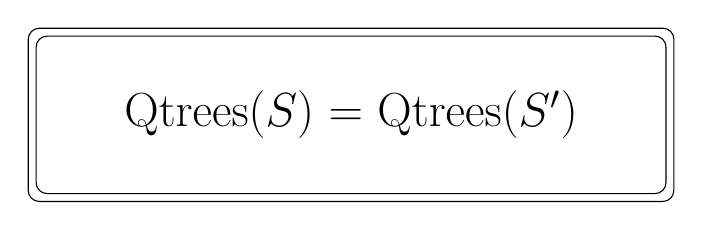
\begin{tikzpicture}
		\draw[rounded corners] (0, 0) rectangle (8, 2) {};
		\draw[rounded corners] (-.1, -.1) rectangle (8.1, 2.1) {};
		\node[] at(4,1) {\LARGE Qtrees($S$) = Qtrees($S'$)};
	\end{tikzpicture}}
	\caption{What a more ``intuitive'' (but inaccurate) version of \textsc{Q-Redundancy} could have been ($S'$ is supposed to be a simplification of $S$).}\label{fig2:redundancy-intuitive-extension}
	\end{subfigure}\hfill
	\begin{subfigure}[b]{.65\linewidth}
		\centering
	\scalebox{.8}{
	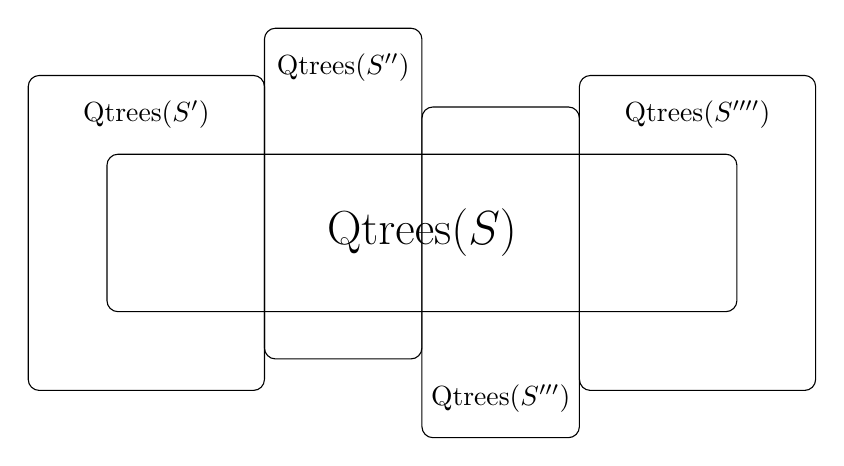
\begin{tikzpicture}
		\draw[rounded corners] (0, 0) rectangle (8, 2) {};
		\draw[rounded corners] (-1, -1) rectangle (2, 3) {};
		\draw[rounded corners] (6, -1) rectangle (9, 3) {};
		\draw[rounded corners] (4, -1.6) rectangle (6, 2.6) {};
		\draw[rounded corners] (2, -.6) rectangle (4, 3.6) {};
		\node[] at(.5,2.5) {Qtrees($S'$)};
		\node[] at(3,3.1) {Qtrees($S''$)};
		\node[] at(5,-1.1) {Qtrees($S'''$)};
		\node[] at(7.5,2.5) {Qtrees($S''''$)};
		\node[] at(4,1) {\LARGE Qtrees($S$)};
	\end{tikzpicture}}
	\caption{What it takes for $S$ to be odd solely due to \textsc{Q-Redundancy} ($S'$, $S''$, $S'''$, and $S''''$ are supposed to be simplifications of $S$).}\label{fig2:q-redundancy}
	\end{subfigure}
	\caption{Comparing \textsc{Q-Redundancy} to a more ``intuitive'' extension of \textsc{Redundancy} to the QuD domain.}
\end{figure}

Our definition of \textsc{Q-Redundancy} also leaves space for other Qtree well-formedness constraints to contribute to a sentence's oddness. For instance, if we also assume, following \citet{HenotMortier2024a}, that \textsc{Relevance} (in the form of \textsc{Q-Relevance}) should filter out Qtrees evoked by sentences, then a sentence may be deemed odd because \textit{some} Qtrees compatible with $S$ can be identified with \textit{some} Qtree generated by \textit{some} simplification of $S$, and the other Qtrees compatible with $S$ are ruled-out by \textsc{Q-Relevance}. This mixed-oddness profile is schematized in Figure \ref{fig2:q-redundancy-relevance}.



\begin{figure}[H]
	\centering
	\scalebox{.8}{
		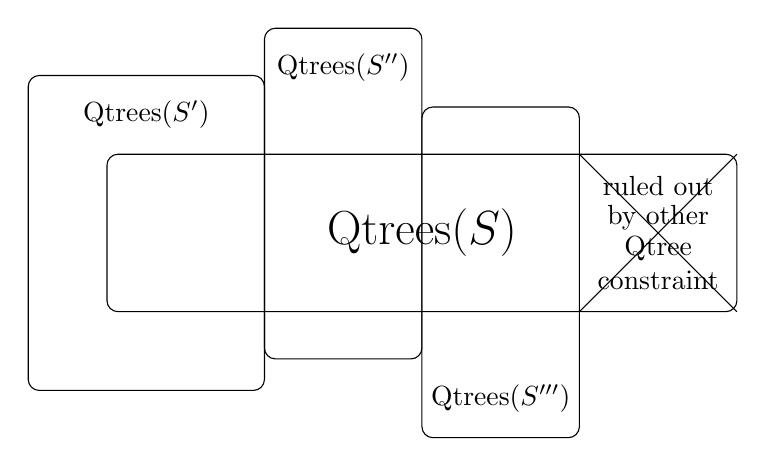
\begin{tikzpicture}
			\draw[rounded corners] (0, 0) rectangle (8, 2) {};
			\draw[rounded corners] (-1, -1) rectangle (2, 3) {};
			\draw[rounded corners] (4, -1.6) rectangle (6, 2.6) {};
			\draw[rounded corners] (2, -.6) rectangle (4, 3.6) {};
			\draw[-] (6,0) -- (8,2);
			\draw[-] (6,2) -- (8,0);
			\node[] at(.5,2.5) {Qtrees($S'$)};
			\node[] at(3,3.1) {Qtrees($S''$)};
			\node[] at(5,-1.1) {Qtrees($S'''$)};
			\node[] at(4,1) {\LARGE Qtrees($S$)};
			\node[] at(7,1.6) {{ruled out}};
			\node[] at(7,1.2) {{by other}};
			\node[] at(7,.8) {{Qtree}};
			\node[] at(7,.4) {{constraint}};
	\end{tikzpicture}}
	\caption{What it means for $S$ to be odd partly due to \textsc{Q-Redundancy}, partly due to other Qtree well-formedness constraints, e.g. \textsc{Q-Relevance}.}\label{fig2:q-redundancy-relevance}
\end{figure}

If \textsc{Q-Redundancy} at the sentential level is not a proper extension of Brevity, \textsc{Q-Redundancy} defined on LF-Qtree pairs (cf. \ref{ex2:q-redundancy}), is. To see this, one must define the simplification of an LF-Qtree pair ($S$, $T$), as a pair ($S'$, $T'$) where $S'$ is a formal simplification of $S$ in the sense of (\ref{ex2:formal-simplification}). Additionally, one must define equivalence between LF-Qtree pairs as equivalence between their Qtree-component. This yields a definition of \textsc{Q-Relevance}-as-Brevity, given in (\ref{ex2:q-redundancy-as-brevity}) that is set as a two-dimensional optimization problem on both LFs (which define conciseness) and Qtrees (which define informativeness).

\begin{exe}
	\ex 
	\begin{xlist}
		\ex {\textit{\textsc{Q-Redundancy} as Brevity on LF-Qtree pairs.} If ($S$, $T$) and ($S'$, $T'$) are two LF-Qtree pairs that are equivalent to each other, then prefer the most concise of the two.}
		\ex {\textit{Conciseness of a LF-Qtree pair.} If ($S$, $T$) and ($S'$, $T'$) are two LF-Qtree pairs, ($S'$, $T'$) is more concise than ($S$, $T$) iff $S'$ is a formal simplification of $S$ as per (\ref{ex2:formal-simplification}).}
		\ex {\textit{Equivalence of a LF-Qtree pair.} If ($S$, $T$) and ($S'$, $T'$) are two LF-Qtree pairs, ($S'$, $T'$) is equivalent to ($S$, $T$) iff $T = T'$.\footnote{This is simplified for the purposes of this paper: equality could be replaced by any more elaborate relation between Qtrees.}}
	\end{xlist}\label{ex2:q-redundancy-as-brevity}
\end{exe}










 
\iffalse
(\ref{ex2:pv(pvq)-repeated}-\ref{ex2:n(pvq)tp-repeated})
(\ref{ex2:pv(pvq)-repeated})
(\ref{ex2:npt(pvq)-repeated})
(\ref{ex2:pv(nptq)-repeated})
(\ref{ex2:pv(nqtp)-repeated})
(\ref{ex2:n(pvq)tp-repeated})
\fi
\section{Exploring extensions and elaborations of the target sentences}\label{sec:exploration}

Before exploring other variations obtained from (\ref{ex2:double-disjunctions}), let us have a word on the slight contrast between (\ref{ex2:pv(nptq)}) and (\ref{ex2:(nptq)vp}), repeated below.

\begin{exe}
	\exr{ex2:pv(nptq)}[] {Either Ido is at SuB or if he is not at SuB then he is in Cambridge.\\ \hfill $\p \vee (\neg \p \rightarrow \q)$}
	\exr{ex2:(nptq)vp}[?] {Either Ido is in Cambridge if not at SuB, or he is at SuB.\\ \hfill $(\neg \p \rightarrow \q) \vee \p$}
\end{exe}

Our account does not predict a contrast between (\ref{ex2:pv(nptq)}) and (\ref{ex2:(nptq)vp}), because disjunction is assumed to have a purely symmetric effect. However, it is possible to assume that, if two forms have same complexity and same accommodated QuDs, the form whose evoked QuD gets incrementally more complex in the course of its computation, should be preferred.

\begin{exe}
	\ex{}
\end{exe}

Q-Redundancy is non-incremental, not only structural. A more surface level redundancy, may be incremental, and structural.



\begin{exe}
	\ex Double \textit{or}-to-\textit{if}
	\begin{xlist}
		\ex[\#] {If Ido is not at SuB then, if he is not at SuB then he is in Cambridge.\hfill $\neg p \rightarrow (\neg p \rightarrow q)$}\label{ex2:nptnptq}
		\ex[\#] {If Ido is not at SuB then, if he is not in Cambridge then he is at SuB.\hfill $\neg p \rightarrow (\neg q \rightarrow p)$}\label{ex2:nptnqtp}
		\ex[] {If it's not that Ido is in Cambridge if not at SuB, then Ido is not at SuB.\hfill $\neg (\neg p \rightarrow q) \rightarrow p$}\label{ex2:nptnqtp}
		\ex[\#] {If it's not that Ido is at SuB if not in Cambridge, then Ido is at SuB.\hfill $\neg (\neg q \rightarrow p) \rightarrow p$}\label{ex2:nptnqtp}
	\end{xlist}
\end{exe}


ido had dessert or cheese and dessert
if ido did not have dessert he had cheese and dessert
if ido did not have cheese and dessert he had dessert

\section{Conclusion and outlook}\label{sec:conclusion}
We presented a set of data based on variation of the redundant structure $p \vee p \vee q$, and showed that the felicity profiles of these sentences was hard to account for, in conjunction with other well known redundant sentences,  
Stress the fact the Hurford Senteces covered by other paper did not allow to deriectly tease apart my account from Kalomoiros' but the sentences at stake in this paper can.





